\fbox{\begin{minipage}[!ht]{38em}

\subsubsection*{(Mis)Fitting: Scaling Law Reproducibility Checklist}


\small

\begin{minipage}[!htp]{0.95\textwidth}
\raggedright
\paragraph{Scaling Law Hypothesis (\S\ref{sec:power-law-form})}

\begin{itemize}[leftmargin=*]
    \item What is the form of the power law? \textit{$L(N, D) = E + \frac{A}{N^\alpha} + \frac{B}{D^\beta} $}
    \item What are the variables related by (included in) the power law? \textit{$N$: the number of model parameters, $D$: the number of data tokens, and $L$: the model's validation loss}
    \item What are the parameters to fit? \textit{$A$, $B$, $E$, $\alpha$, $\beta$}
    \item On what principles is this form derived? \textit{This is taken from \citet{hoffmann2022training}, who hypothesize this form on the basis of prior work in risk decomposition.}
    \item Does this form make assumptions about how the variables are related? \textit{This form inherently assumes that $N$ and $D$ do not have any interaction in their effect on the scaling of $L$. For some experiments, we use the assumption $\alpha = \beta$ to simplify optimization.}
    % \item How are each of these variables counted? (For example, how is compute cost/FLOPs counted, if applicable? How are parameters of the model counted?)
    % \item Are code/code snippets provided for calculating these variables if applicable? 
\end{itemize}


\paragraph{Training Setup (\S\ref{sec:model_training})}
\begin{itemize}[leftmargin=*]
    \item How many models are trained?
    \textit{Refer to Table 10}
    \item At which sizes?
    \textit{Refer to Table 10}
    \item On how much data each? On what data? Is any data repeated within the training for a model?
    \textit{Refer to Table 10.}
    \item How are model size, dataset size, and compute budget size counted? For example, how are parameters of the model counted? Are any parameters excluded (e.g., embedding layers)? How is compute cost calculated?  \textit{We include the results including and excluding embedding layers for both the total parameter count $N$ and the total FLOP count $C$. We also include, for comparison, results using the estimate $C=6ND$.}
    \item Are code/code snippets provided for calculating these variables if applicable?
    \url{https://github.com/hadasah/scaling_laws}
    \item How are hyperparameters chosen (e.g., optimizer, learning rate schedule, batch size)? Do they change with scale? \textit{Most hyperparameters are chosen based on best practices in current literature; several are taken directly from the settings in \citet{hoffmann2022training}. For learning rate, we conduct an extensive hyperparameter search across 2-3 orders of magnitude, multiplying by 2-2.5, and then conduct training at 3 learning rates, including the optimum, for nearly all ($N$, $D$) configurations.}
    \item What other settings must be decided (e.g., model width vs. depth)? Do they change with scale?  
    \textit{Refer to Table 10}
    \item Is the training code open source?
    \textit{Yes}
\end{itemize}


\begin{figure*}[t]
    \centering
    \small
    \hspace*{-1.2cm}
    \subfigure[Alignment stage]{
    \begin{minipage}[t]{0.24\linewidth}
    \centering
      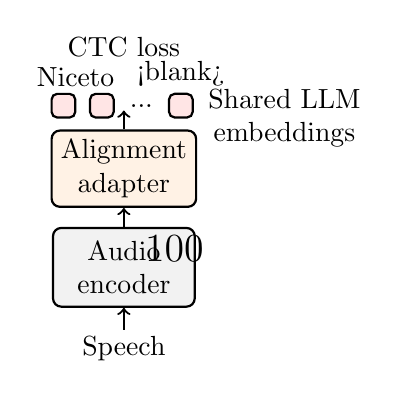
\begin{tikzpicture} [scale=0.8]
        \node(ae) at (0,0) [rectangle, draw=black, fill=gray!10, rounded corners=3pt, thick, minimum width=1.8cm,minimum height=1cm,align=center] {Audio\\encoder};
        \node(freeze) at ([xshift=0.8cm,yshift=0.3cm]ae.center) [rectangle, align=center] {\Large{\ding{100}}};
        \node(fb) at ([yshift=-0.3cm]ae.south) [rectangle, align=center,anchor=north] {Speech};
        \node(aa) at ([yshift=0.3cm]ae.north) [rectangle, draw=black, fill=orange!10, rounded corners=3pt, thick, minimum width=1.8cm,minimum height=0.5cm,align=center,anchor=south] {Alignment\\adapter};
        
        \node(f1) at ([yshift=1.0cm]aa.west) [rectangle, draw=black, fill=red!10, rounded corners=2pt, thick, minimum width=0.3cm, minimum height=0.3cm,align=center,anchor=west] {};
        \node(f2) at ([xshift=0.2cm]f1.east) [rectangle, draw=black, fill=red!10, rounded corners=2pt, thick, minimum width=0.3cm, minimum height=0.3cm,align=center,anchor=west] {};
        \node(f3) at ([xshift=0.075cm]f2.east) [rectangle, draw=white,  thick, align=center,anchor=west] {...};
        \node(f4) at ([xshift=0.075cm]f3.east) [rectangle, draw=black, fill=red!10, rounded corners=2pt, thick, minimum width=0.3cm, minimum height=0.3cm,align=center,anchor=west] {};
        \node(t1) at ([yshift=-0.05cm]f1.north) [rectangle, align=center,anchor=south] {Nice};
        \node(t2) at ([yshift=-0.05cm]f2.north) [rectangle, align=center,anchor=south] {to};
        \node(t4) at ([yshift=-0.05cm]f4.north) [rectangle, align=center,anchor=south] {<blank>};
        \node(se) at ([xshift=0.075cm,yshift=-0.2cm]f4.east) [rectangle, align=center,anchor=west] {Shared LLM\\embeddings};
        \node(ctc) at ([yshift=1.0cm]aa.north) [rectangle, rounded corners=3pt, thick, align=center,anchor=south] {CTC loss};

        
        \draw[->,thick]([yshift=-0.05cm]fb.north)--(ae.south);
        \draw[->,thick](ae.north)--(aa.south);
        \draw[->,thick](aa.north)--([yshift=0.3cm]aa.north);

        
      \end{tikzpicture}
    \end{minipage}
    }
    \subfigure[Shrinking stage]{
    \begin{minipage}[t]{0.45\linewidth}
    \centering
    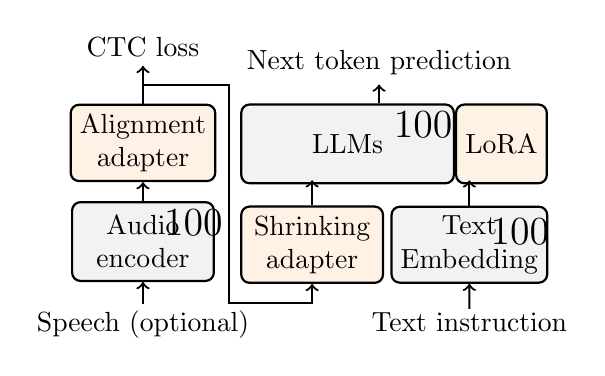
\begin{tikzpicture} [scale=0.8]
        \node(ae) at (0,0) [rectangle, draw=black, fill=gray!10, rounded corners=3pt, thick, minimum width=1.8cm,minimum height=1cm,align=center] {Audio\\encoder};
        \node(freeze) at ([xshift=0.8cm,yshift=0.3cm]ae.center) [rectangle, align=center] {\Large{\ding{100}}};
        \node(fb) at ([yshift=-0.3cm]ae.south) [rectangle, align=center,anchor=north] {Speech (optional)};
        \node(aa) at ([yshift=0.3cm]ae.north) [rectangle, draw=black, fill=orange!10, rounded corners=3pt, thick, minimum width=1.8cm,minimum height=0.5cm,align=center,anchor=south] {Alignment\\adapter};
        \node(ctc) at ([yshift=0.6cm]aa.north) [rectangle,align=center,anchor=south] {CTC loss};
        \node(sa) at ([xshift=0.4cm,yshift=-0.05cm]ae.east) [rectangle, draw=black, fill=orange!10, rounded corners=3pt, thick, minimum width=1.8cm,minimum height=0.5cm,align=center,anchor=west] {Shrinking\\adapter};
        \node(llm) at ([yshift=1.6cm]sa.west) [rectangle, draw=black, fill=gray!10, rounded corners=3pt, thick, minimum width=2.7cm,minimum height=1.0cm,align=center,anchor=west] {LLMs};
        \node(lora) at (llm.east) [rectangle, draw=black, fill=orange!10, rounded corners=3pt, thick, minimum width=1.0cm,minimum height=1.0cm,align=center,anchor=west] {LoRA};
        \node(te) at ([xshift=0.1cm]sa.east) [rectangle, draw=black, fill=gray!10, rounded corners=3pt, thick, minimum width=1.8cm,minimum height=0.5cm,align=center,anchor=west] {Text\\Embedding};
        \node(freeze3) at ([xshift=0.8cm,yshift=0.2cm]te.center) [rectangle, align=center] {\Large{\ding{100}}};
        \node(ti) at ([yshift=-0.3cm]te.south) [rectangle, align=center,anchor=north] {Text instruction};
        \node(freeze2) at ([xshift=1.2cm,yshift=0.3cm]llm.center) [rectangle, align=center] {\Large{\ding{100}}};
        \node(loss) at ([xshift=0.5cm, yshift=0.3cm]llm.north) [rectangle, align=center,anchor=south] {Next token prediction};

        
        \draw[->,thick]([yshift=-0.05cm]fb.north)--(ae.south);
        \draw[->,thick](ae.north)--(aa.south);
        \draw[->,thick](aa.north)--(ctc.south);
        \draw[->,thick](sa.north)--([yshift=0.4cm]sa.north);
        \draw[->,thick](te.north)--([yshift=0.4cm]te.north);
        \draw[->,thick]([yshift=-0.3cm]loss.south)--(loss.south);
        \draw[->,thick]([yshift=-0.1cm]ti.north)--(te.south);

        \draw[->,thick](aa.north)--([yshift=0.3cm]aa.north)--([xshift=0.2cm, yshift=0.3cm]aa.north -| aa.east)--([xshift=0.2cm, yshift=-0.3cm]sa.south -| aa.east)--([yshift=-0.3cm]sa.south)--(sa.south);
      \end{tikzpicture}
    \end{minipage}
    }
    \subfigure[SFT stage]{
    \begin{minipage}[t]{0.20\linewidth}
    \centering
    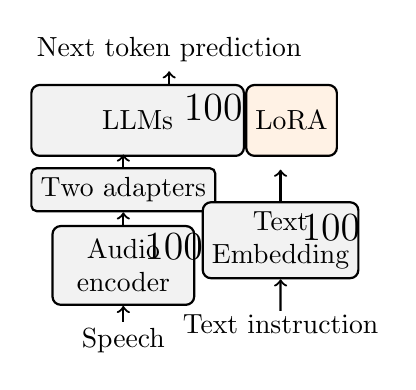
\begin{tikzpicture} [scale=0.8]
        \node(ae) at (0,0) [rectangle, draw=black, fill=gray!10, rounded corners=3pt, thick, minimum width=1.8cm,minimum height=1cm,align=center] {Audio\\encoder};
        \node(freeze) at ([xshift=0.8cm,yshift=0.3cm]ae.center) [rectangle, align=center] {\Large{\ding{100}}};
        \node(fb) at ([yshift=-0.2cm]ae.south) [rectangle, align=center,anchor=north] {Speech};
        \node(aa) at ([yshift=0.2cm]ae.north) [rectangle, draw=black, fill=gray!10, rounded corners=2pt, thick, minimum width=1.8cm,minimum height=0.5cm,align=center,anchor=south] {Two adapters};
        
        \node(llm) at ([yshift=1.1cm]aa.west) [rectangle, draw=black, fill=gray!10, rounded corners=3pt, thick, minimum width=2.7cm,minimum height=0.9cm,align=center,anchor=west] {LLMs};
        \node(lora) at (llm.east) [rectangle, draw=black, fill=orange!10, rounded corners=3pt, thick, minimum width=0.9cm,minimum height=0.9cm,align=center,anchor=west] {LoRA};
        \node(te) at ([xshift=0.1cm,yshift=0.4cm]ae.east) [rectangle, draw=black, fill=gray!10, rounded corners=3pt, thick, minimum width=1.8cm,minimum height=0.5cm,align=center,anchor=west] {Text\\Embedding};
        \node(freeze3) at ([xshift=0.8cm,yshift=0.2cm]te.center) [rectangle, align=center] {\Large{\ding{100}}};
        \node(ti) at ([yshift=-0.4cm]te.south) [rectangle, align=center,anchor=north] {Text instruction};
        \node(freeze2) at ([xshift=1.2cm,yshift=0.2cm]llm.center) [rectangle, align=center] {\Large{\ding{100}}};
        \node(loss) at ([xshift=0.5cm, yshift=0.2cm]llm.north) [rectangle, align=center,anchor=south] {Next token prediction};
       
        \draw[->,thick]([yshift=-0.05cm]fb.north)--(ae.south);
        \draw[->,thick](ae.north)--(aa.south);
        \draw[->,thick](aa.north)--([yshift=0.2cm]aa.north);
        \draw[->,thick](te.north)--([yshift=0.5cm]te.north);
        \draw[->,thick]([yshift=-0.2cm]loss.south)--(loss.south);
        \draw[->,thick]([yshift=-0.1cm]ti.north)--(te.south);
        
      \end{tikzpicture}
    \end{minipage}
    }
      \caption{Training progress of Soundwave. The gray modules are frozen while the orange modules are updated.}
      \label{architecture}
  \end{figure*}

  

\raggedright

\end{minipage}

\end{minipage}}

\fbox{\begin{minipage}[!ht]{38em}

\small

\begin{minipage}[!ht]{0.9\textwidth}
\raggedright

\paragraph{Data Collection(\S\ref{sec:data})}
\begin{itemize}[leftmargin=*]
    \item Are the model checkpoints provided openly?
    % \item Are these checkpoints modified in any way before evaluation? (say, checkpoint averaging)
    % \item If the above is done, is code for modifying the checkpoints provided?
    \textit{Yes, at  \url{https://github.com/hadasah/scaling_laws}}
    \item How many checkpoints per model are evaluated to fit each scaling law? Which ones, if so?  \textit{Unless clearly denoted otherwise, one checkpoint per model is evaluated; the last checkpoint. By default, no mid-training checkpoints are used, i.e., from before the termination of the cosine learning rate schedules.}
    \item What evaluation metric is used? On what dataset?  \textit{We use cross-entropy loss, measured on a held-out validation subset of the Common Crawl \citep{raffel2020exploring} dataset.}
    \item Are the raw evaluation metrics modified? Some examples include loss interpolation, centering around a mean or scaling logarithmically.  \textit{No.}
    \item If the above is done, is code for modifying the metric provided? 
    \textit{Yes.}
\end{itemize}


\paragraph{Fitting Algorithm (\S\ref{sec:opt})}
\begin{itemize}[leftmargin=*]
    \item What objective (loss) is used? \textit{We try various loss objectives (1) log-Huber loss, (2) MSE, (3) MAE and (4) Huber loss}
    \item What algorithm is used to fit the equation? \textit{Mainly L-BFGS, but we also experiment with BFGS, non-linear least squares and grid search.}
    \item What hyperparameters are used for this algorithm? \textit{Thresholds of $\{1e-4, 1e-6, 1e-8\}$, exact gradient }
    \item How is this algorithm initialized? \textit{We initialize with 4500 initializations similar to \citet{hoffmann2022training}.}
    \item Are all datapoints collected used to fit the equations? For example, are any outliers dropped? Are portions of the datapoints used to fit different equations? \textit{No outliers are dropped in general, but we do show some results on specific subsets of models. For example, we compare the result of a scaling law fit when using only models trained at a peak learning rate of $1e-4$ or $4e-4$.}
    \item How is the correctness of the scaling law considered? Extrapolation, Confidence Intervals, Goodness of Fit? \textit{Currently, we do not evaluate the correctness beyond comparing to results in literature \citep{hoffmann2022training,kaplan2020scaling}.}
\end{itemize}

\end{minipage}

% \paragraph{Other}
% \begin{itemize}
%     \item Is code for 
% \end{itemize}

\end{minipage}}